\chapter{Resultados e Discussão}
\label{cap:resultados}

\section{Análise Exploratória dos Dados}
\label{cap:resultados:sec:analise_exploratoria}

Foram identificados 814 hotéis distribuídos em todo o território nacional, desde hotéis de grandes redes e com disponibilidade de reservas do tipo \textit{All Inclusive} até hotéis pouco conhecidos com menos de 10 avaliações na plataforma.

Dessa lista temos como destaque os seguintes números:

Estados com a maior quantidade de hotéis
\begin{itemize}
	\item RJ: 71
	\item SP: 67
	\item PA: 62
	\item MG: 61
	\item RR/PI/MS: 60
\end{itemize}

Estados com a maior quantidade de avaliações

\begin{itemize}
	\item RJ: 231947 (4,22 com 71 hotéis)
	\item SP: 169586 (4,21 com 67 hotéis)
	\item BA: 107716 (4,34 com 22 hotéis)
	\item MG: 107067 (4,35 com 61 hotéis)
	\item PB: 68188 (4,36 com 54 hotéis)
\end{itemize}

Média da classificação dos hotéis por Estado

\begin{itemize}
	\item RS: 4,70 com 9493 avaliações no total (2 hotéis)
	\item AL: 4,64 com 33345 avaliações no total (8 hotéis)
	\item AC: 4,60 com 1696 avaliações no total (1 hotel)
	\item AM: 4,53 com 45509 avaliações no total (46 hotéis)
	\item SC: 4,50 com 32621 avaliações no total (7 hotéis)
\end{itemize}

Após aplicar o primeiro critério definido para a seleção da lista de hotéis, temos então uma lista com um grupo de 15 hotéis dentre os disponíveis, e após o filtro da região temos então 11. Também foram adicionados manualmente a lista outros 2 hotéis que atendiam os critérios hotéis que não foram listados nas consultas à \textit{API}.

A lista composta de 13 hotéis todos localizados na região nordeste do Brasil e com a disponibilidade de pacotes \textit{All Inclusive}, conforme tabela~\ref{table:lista_hoteis}, é valido notar que todos os hotéis da lista no momento da escolha possuíam uma avaliação na plataforma do \textit{Google Maps} com nota igual ou superior a 4,20 e são todos hotéis apontados pela plataforma como sendo hotéis de classificação de 4 ou 5 estrelas.

\begin{table}[]
	\begin{tabular}{|p{5cm}|l|r|r|l|r|}
		\hline
		\textbf{Nome}                                 & \textbf{Estado} & \textbf{Nota} & \textbf{Estrelas} & \textbf{Região} & \textbf{Quantidade} \\\hline
		Cana Brava All Inclusive Resort               & BA              & 4.60          & 4                 & NORDESTE        & 10987               \\\hline
		Grand Oca Maragogi                            & AL              & 4.30          & 5                 & NORDESTE        & 4613                \\\hline
		Hotel Marsol Beach Resort                     & RN              & 4.20          & 4                 & NORDESTE        & 3269                \\\hline
		Hotel Vila Galé - Touros                      & RN              & 4.60          & 5                 & NORDESTE        & 5619                \\\hline
		Hotel Vila Galé - Marés                       & BA              & 4.50          & 5                 & NORDESTE        & 8516                \\\hline
		Hotel Vila Galé: Eco Resort - Cabo            & PE              & 4.50          & 5                 & NORDESTE        & 5370                \\\hline
		Iberostar Bahia                               & BA              & 4.70          & 5                 & NORDESTE        & 16109               \\\hline
		La Torre Resort All Inclusive                 & BA              & 4.70          & 4                 & NORDESTE        & 6140                \\\hline
		Makai Resort Aracaju - All Inclusive          & SE              & 4.30          & 4                 & NORDESTE        & 5276                \\\hline
		Nauticomar Resort All Inclusive \& Beach Club & BA              & 4.30          & 4                 & NORDESTE        & 4258                \\\hline
		Salinas Maceió All Inclusive Resort           & AL              & 4.70          & 4                 & NORDESTE        & 4663                \\\hline
		Salinas Maragogi All Inclusive Resort         & AL              & 4.80          & 5                 & NORDESTE        & 7111                \\\hline
		Transamerica Comandatuba                      & BA              & 4.80          & 4                 & NORDESTE        & 3179                \\\hline
	\end{tabular}%
	\caption{Lista de hotéis e número de avaliações}
	\label{table:lista_hoteis}
\end{table}

\begin{figure}
	\centering
	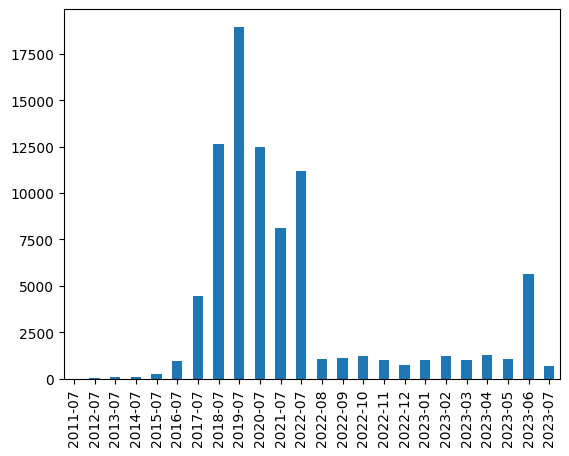
\includegraphics[width=0.75\textwidth]{figs/exploratoria/distribuicao_ano_mes_avaliacao.png}
	\caption{Distribuição do número de avaliação por mês e ano}
	\label{img:dist_ano_mes_avaliacao}
\end{figure}

Tratamos então os dados de avaliações e agora possuímos a nova coluna \textit{mes\_ano\_avaliacao}, na Figura \ref{img:dist_ano_mes_avaliacao}, nota-se um comportamento estranho com a ausência de diversos meses por ano, durante o período de 2011 até 2021 temos o registro de apenas avaliações no mês 7, este comportamento é devido ao formato de data relativa utilizada pelo \textit{Google Maps} ao expor suas avaliações, não foi possível identificar uma forma de adquirir o tempo definitivo de quando a avaliação foi publicada.

Por este motivo ao se utilizar a data relativa passamos a ter dificuldade com as avaliações mais antigas, e conseguimos apenas identificar o ano no qual a avaliação foi publicada, as avaliações com menos de um ano de diferença da data de recuperação e utilizando este \textit{script} poderiam ser utilizadas em uma análise mais detalhada em relação ao período, porém esta não será a estratégia adotada e optaremos por restringir a análise de maneira que as avaliações serão agrupadas em períodos anuais, representando assim o ano de publicação de cada avaliação.

\begin{table}[]
	\centering
	\begin{tabular}{|l|l|}
		\hline
		\textbf{Ano} & \textbf{Quantidade} \\\hline
		2023         & 11925               \\
		2022         & 16364               \\
		2021         & 8104                \\
		2020         & 12489               \\
		2019         & 18963               \\
		2018         & 12625               \\
		2017         & 4426                \\
		2016         & 940                 \\
		2015         & 247                 \\
		2014         & 106                 \\
		2013         & 88                  \\
		2011         & 5                   \\
		2012         & 9                   \\
		\hline
	\end{tabular}%
	\caption{Quantidade de avaliações obtidas por ano}
	\label{table:review_per_year}
\end{table}

Considerando todas as avaliações obtidas podemos observar na tabela~\ref{table:review_per_year} que temos uma discrepância na quantidade e é perceptível a divisão no período de 2017/2018.

E dessa forma foi definido que serão utilizadas avaliações posteriores a 2018.

Resultando um código conforme abaixo:

\lstinputlisting[language=Python,caption=Filtros aplicados ao dataset de avalições]{extras/code/review_filter.py}

Considerando todas as avaliações obtidas, temos:

\begin{itemize}
	\item 80470(93.25\%) enviadas depois de 2017 e 5821(6.75\%) enviadas em 2017, ou antes
	\item 56893(65.93\%) com texto e 3 ou mais caracteres, 29386(34.05\%) sem texto e 12(0.01\%) avaliações com 1 ou 2 caracteres
	\item 4184(4.85\%) avaliações traduzidas
\end{itemize}

Agora estamos considerando apenas avaliações que serão utilizadas na análise, a distribuição das notas atribuídas individualmente a cada avaliação pode ser consultada na Figura \ref{img:dist_review_rating}. É fácil notar que a grande maioria das avaliações registradas, mais especificamente 38347 (77,91\%), possui a maior nota atribuída, de valor 5, o que nos leva a acreditar que na maioria das avaliações o sentimento geral que deve ser identificado será positivo.

\begin{figure}
	\centering
	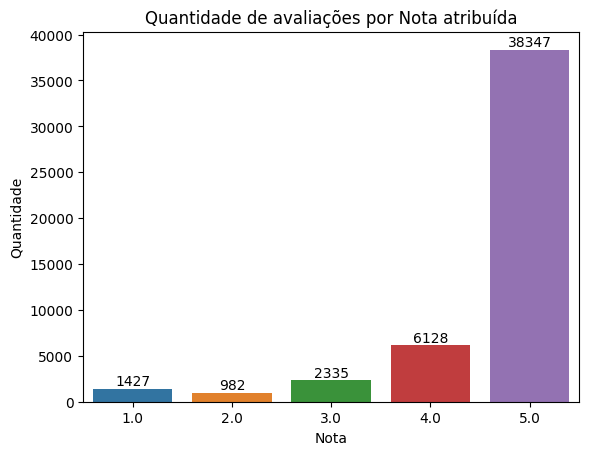
\includegraphics[width=0.75\textwidth]{figs/exploratoria/quantidade_avaliacao_nota_atribuida.png}
	\caption{Quantidade de avaliações por nota atribuída}
	\label{img:dist_review_rating}
\end{figure}

Este comportamento de distribuição desigual das notas ainda é perceptível também quando olhamos para as avaliações agrupadas por ano de submissão, como se pode notar na Figura \ref{img:dist_review_rating_per_year}. Podemos também observar na Figura \ref{img:dist_review_rating_per_year} a evolução em quantidade numérica durante o tempo, podendo notar uma quebra de tendência no crescimento pós 2019, nos anos de 2020 e 2021, provavelmente causado pelo confinamento decorrente da COVID-19~\cite{Guardia2022} e já pós-flexibilização do confinamento, 2022, visualizamos um aumento expressivo no número de avaliações, levando ainda em consideração que temos apenas 6 meses de avaliação em 2023 então seguiremos possivelmente com a tendência de aumento de número de avaliações ano após ano provavelmente 2023 será o ano com maior número de avaliações.

\begin{figure}
	\centering
	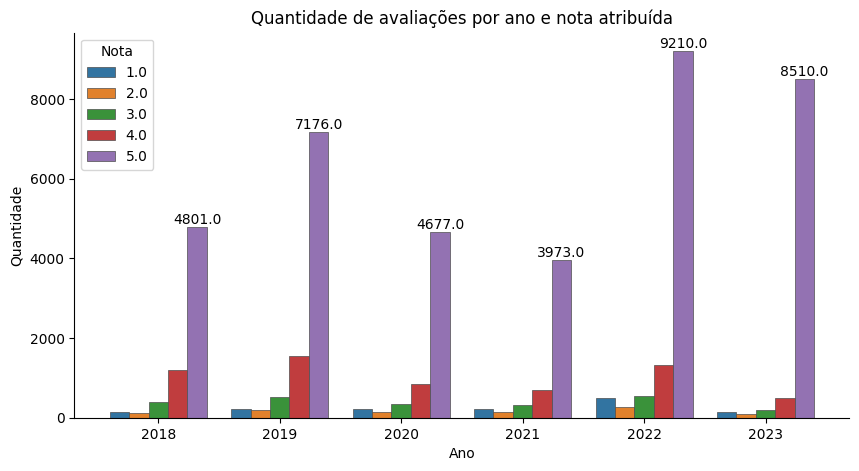
\includegraphics[width=1\textwidth]{figs/exploratoria/quantidade_avaliacao_nota_atribuida_ano.png}
	\caption{Quantidade de avaliações por ano e nota atribuída}
	\label{img:dist_review_rating_per_year}
\end{figure}

Com a Figura \ref{img:relplot_ano_rating} podemos notar que a variação da nota atribuída tende a diminuir conforme o tempo passa, pois a quantidade de notas maiores é cresce de forma desproporcional se comparado com as avaliações com notas baixas, como observado na Figura \ref{img:dist_review_rating_per_year}.

% \begin{figure}
% 	\centering
% 	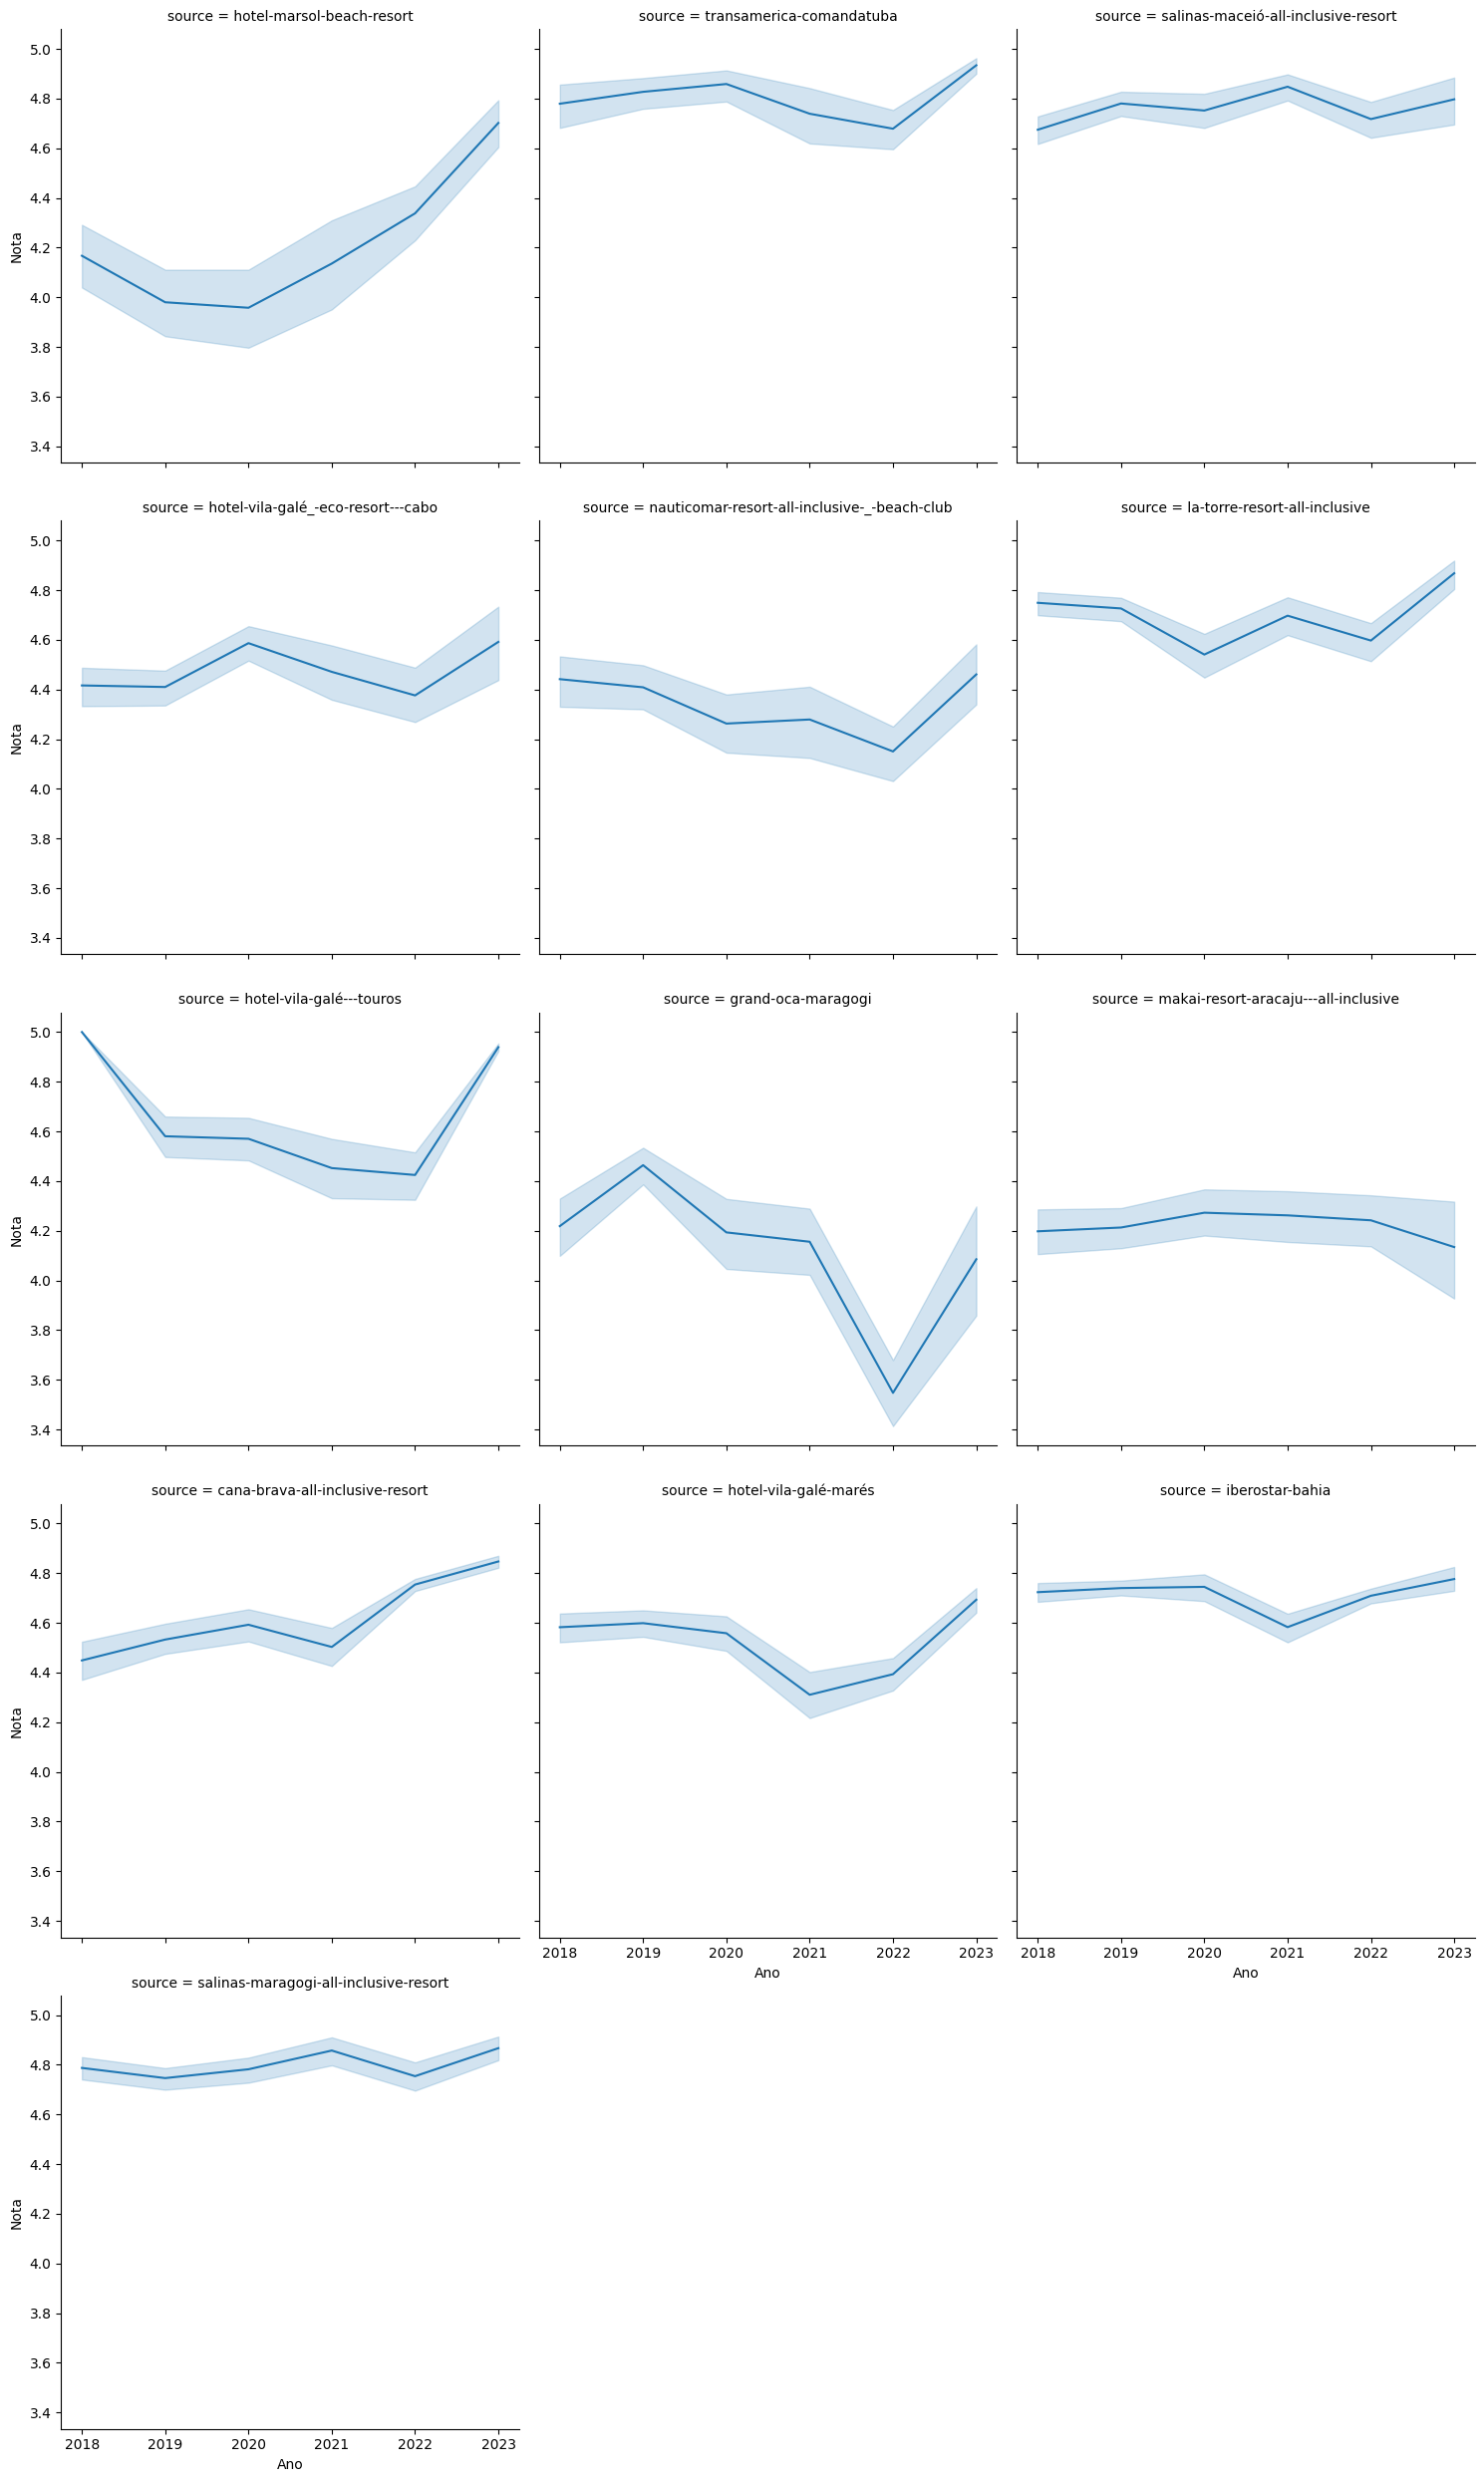
\includegraphics[width=1\textwidth]{figs/exploratoria/relplot_ano_rating_source.png}
% 	\caption{Variação da nota atribuída ao longo dos anos por hotel}
% 	\label{img:relplot_ano_rating_source}
% \end{figure}

\begin{table}[]
	\centering
	\begin{tabular}{|p{5cm}|l|l|l|l|}
		\hline
		\textbf{Hotel}                                      &
		\textbf{Não vazio}                                  &
		\textbf{Com texto}                                  &
		\textbf{Traduzido}                                  &
		\textbf{Públicos em +2017}                            \\
		\hline
		\textbf{Cana Brava All Inclusive Resort}            &
		8583                                                &
		8581                                                &
		141                                                 &
		10656                                                 \\
		\hline
		\textbf{Grand Oca Maragogi}                         &
		2948                                                &
		2947                                                &
		542                                                 &
		4297                                                  \\
		\hline
		\textbf{Hotel Marsol Beach Resort}                  &
		2150                                                &
		2150                                                &
		162                                                 &
		3128                                                  \\
		\hline
		\textbf{Hotel Vila Galé - Touros}                   &
		4481                                                &
		4480                                                &
		111                                                 &
		5802                                                  \\
		\hline
		\textbf{Hotel Vila Galé - Marés}                    &
		5723                                                &
		5721                                                &
		315                                                 &
		7981                                                  \\
		\hline
		\textbf{Hotel Vila Galé Eco Resort - Cabo}          &
		3219                                                &
		3217                                                &
		183                                                 &
		4934                                                  \\
		\hline
		\textbf{Iberostar Bahia}                            &
		10587                                               &
		10586                                               &
		1464                                                &
		14848                                                 \\
		\hline
		\textbf{La Torre Resort - All Inclusive}            &
		3847                                                &
		3847                                                &
		496                                                 &
		5722                                                  \\
		\hline
		\textbf{Makai Resort Aracaju - All Inclusive}       &
		3180                                                &
		3180                                                &
		84                                                  &
		4917                                                  \\
		\hline
		\textbf{Nauticomar Resort All Inclusive Beach Club} &
		2630                                                &
		2628                                                &
		228                                                 &
		3938                                                  \\
		\hline
		\textbf{Salinas Maceió All Inclusive Resort}        &
		2836                                                &
		2836                                                &
		168                                                 &
		4497                                                  \\
		\hline
		\textbf{Salinas Maragogi All Inclusive Resort}      &
		4572                                                &
		4572                                                &
		203                                                 &
		6700                                                  \\
		\hline
		\textbf{Transamerica Comandatuba}                   &
		2149                                                &
		2148                                                &
		87                                                  &
		3050                                                  \\ \hline
	\end{tabular}
	\caption{Quantidade de avaliações em cada filtro pro hotél}
	\label{table:qtd_review_filtro}
\end{table}

\begin{table}[h]
	\centering
	\begin{tabular}{|c|crrrrr|}
		\hline
		\multicolumn{1}{|c|}{\multirow{2}{*}{\textbf{Estado}}} &
		\multicolumn{2}{c|}{\textbf{analisar}}                 &
		\multicolumn{3}{c|}{\textbf{nota}}                     &
		\multicolumn{1}{c|}{\textbf{estrelas}}                                                                            \\ \cline{2-7}
		\multicolumn{1}{|l|}{}                                 &
		\multicolumn{1}{c}{\textbf{rotulo}}                    &
		\multicolumn{1}{c|}{\textbf{quantidade}}               &
		\multicolumn{1}{c}{\textbf{média}}                     &
		\multicolumn{1}{c}{\textbf{min}}                       &
		\multicolumn{1}{c|}{\textbf{max}}                      &
		\multicolumn{1}{c|}{\textbf{média}}                                                                               \\ \hline
		\multirow{2}{*}{\textbf{AL}}                           & \textbf{False} & 8106  & 4.623896 & 4.3 & 4.8 & 4.735998 \\
		                                                       & \textbf{True}  & 8668  & 4.643205 & 4.3 & 4.8 & 4.706853 \\ \hline
		\multirow{2}{*}{\textbf{BA}}                           & \textbf{False} & 20970 & 4.617740 & 4.3 & 4.8 & 4.542680 \\
		                                                       & \textbf{True}  & 28727 & 4.613016 & 4.3 & 4.8 & 4.467017 \\ \hline
		\multirow{2}{*}{\textbf{PE}}                           & \textbf{False} & 2645  & 4.500000 & 4.5 & 4.5 & 5.000000 \\
		                                                       & \textbf{True}  & 2746  & 4.500000 & 4.5 & 4.5 & 5.000000 \\ \hline
		\multirow{2}{*}{\textbf{RN}}                           & \textbf{False} & 2903  & 4.397451 & 4.2 & 4.6 & 4.493627 \\
		                                                       & \textbf{True}  & 6232  & 4.480424 & 4.2 & 4.6 & 4.701059 \\ \hline
		\multirow{2}{*}{\textbf{SE}}                           & \textbf{False} & 2448  & 4.300000 & 4.3 & 4.3 & 4.000000 \\
		                                                       & \textbf{True}  & 2846  & 4.300000 & 4.3 & 4.3 & 4.000000 \\ \hline
	\end{tabular}\caption{Quantidade de avaliações por estado e por rotulo -- indicando o que será e o que não será analisado}
	\label{table:distribuicao_review_por_estado}
\end{table}

E dentre todas as avaliações obtidas após aplicar o filtro de período utilizaremos para a análise o total de 49219(57.04\%) e 37072(42.96\%) foram ignoradas. Assim as avaliações que foram consideradas estão então distribuídas conforme a tabela~\ref{table:distribuicao_review_per_year}.

\begin{table}[h]
	\centering
	\begin{tabular}{|l|l|}
		\hline
		\textbf{Ano} & \textbf{Quantidade} \\\hline
		2023         & 9444                \\
		2022         & 11866               \\
		2021         & 5350                \\
		2020         & 6236                \\
		2019         & 9645                \\
		2018         & 6678                \\
		\hline
	\end{tabular}
	\caption{Quantidade de avaliações por ano após filtro}
	\label{table:distribuicao_review_per_year}
\end{table}

% TODO

\begin{table}[h]
	\centering
	\begin{tabular}{|c|c|r|r|}
		\hline
		\multicolumn{1}{|r|}{\textbf{Hotel}}                                    &
		\multicolumn{1}{r|}{\textbf{Analisar?}}                                 &
		\textbf{Quantidade}                                                     &
		\textbf{\%}                                                               \\ \hline
		\multirow{2}{*}{\textbf{Cana Brava All Inclusive Resort}}               &
		False                                                                   &
		3028                                                                    &
		27.16                                                                     \\ \cline{2-4}
		                                                                        &
		True                                                                    &
		8119                                                                    &
		72.84                                                                     \\ \hline
		\multirow{2}{*}{\textbf{Grand Oca Maragogi}}                            &
		False                                                                   &
		2427                                                                    &
		52.34                                                                     \\ \cline{2-4}
		                                                                        &
		True                                                                    &
		2210                                                                    &
		47.66                                                                     \\ \hline
		\multirow{2}{*}{\textbf{Hotel Marsol Beach Resort}}                     &
		False                                                                   &
		1470                                                                    &
		44.10                                                                     \\ \cline{2-4}
		                                                                        &
		True                                                                    &
		1863                                                                    &
		55.90                                                                     \\ \hline
		\multirow{2}{*}{\textbf{Hotel Vila Galé - Touros}}                      &
		False                                                                   &
		1433                                                                    &
		24.70                                                                     \\ \cline{2-4}
		                                                                        &
		True                                                                    &
		4369                                                                    &
		75.30                                                                     \\ \hline
		\multirow{2}{*}{\textbf{Hotel Vila Galé - Marés}}                       &
		False                                                                   &
		3550                                                                    &
		41.36                                                                     \\ \cline{2-4}
		                                                                        &
		True                                                                    &
		5033                                                                    &
		58.64                                                                     \\ \hline
		\multirow{2}{*}{\textbf{Hotel Vila Galé: Eco Resort - Cabo}}            &
		False                                                                   &
		2645                                                                    &
		49.06                                                                     \\ \cline{2-4}
		                                                                        &
		True                                                                    &
		2746                                                                    &
		50.94                                                                     \\ \hline
		\multirow{2}{*}{\textbf{Iberostar Bahia}}                               &
		False                                                                   &
		7830                                                                    &
		48.29                                                                     \\ \cline{2-4}
		                                                                        &
		True                                                                    &
		8383                                                                    &
		51.71                                                                     \\ \hline
		\multirow{2}{*}{\textbf{La Torre Resort All Inclusive}}                 &
		False                                                                   &
		3164                                                                    &
		50.84                                                                     \\ \cline{2-4}
		                                                                        &
		True                                                                    &
		3060                                                                    &
		49.16                                                                     \\ \hline
		\multirow{2}{*}{\textbf{Makai Resort Aracaju - All Inclusive}}          &
		False                                                                   &
		2448                                                                    &
		46.24                                                                     \\ \cline{2-4}
		                                                                        &
		True                                                                    &
		2846                                                                    &
		53.76                                                                     \\ \hline
		\multirow{2}{*}{\textbf{Nauticomar Resort All Inclusive \& Beach Club}} &
		False                                                                   &
		2104                                                                    &
		49.03                                                                     \\ \cline{2-4}
		                                                                        &
		True                                                                    &
		2187                                                                    &
		50.97                                                                     \\ \hline
		\multirow{2}{*}{\textbf{Salinas Maceió All Inclusive Resort}}           &
		False                                                                   &
		2140                                                                    &
		45.72                                                                     \\ \cline{2-4}
		                                                                        &
		True                                                                    &
		2541                                                                    &
		54.28                                                                     \\ \hline
		\multirow{2}{*}{\textbf{Salinas Maragogi All Inclusive Resort}}         &
		False                                                                   &
		3539                                                                    &
		47.46                                                                     \\ \cline{2-4}
		                                                                        &
		True                                                                    &
		3917                                                                    &
		52.54                                                                     \\ \hline
		\multirow{2}{*}{\textbf{Transamerica Comandatuba}}                      &
		False                                                                   &
		1294                                                                    &
		39.95                                                                     \\ \cline{2-4}
		                                                                        &
		True                                                                    &
		1945                                                                    &
		60.05                                                                     \\ \hline
	\end{tabular}
	\caption{Lista de quantidade de avaliações analisadas e descartadas por hotel}
	\label{tab:lista_review_hoteis}
\end{table}

Após devido tratamento das avaliações conseguimos obter as nuvens de palavras considerando todas as palavras na Figura \ref{img:wordcloud_geral}, onde podemos notar como alguns dos destaques quarto, piscina, praia, restaurante, como sendo as palavras com maior frequência nas avaliações.

\begin{figure}
	\centering
	\begin{minipage}{0.45\textwidth}
		\centering
		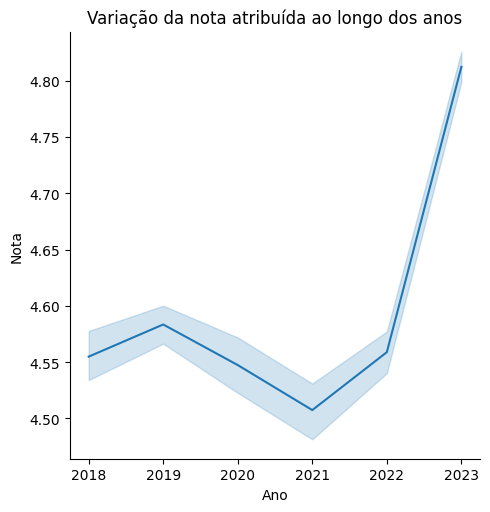
\includegraphics[width=1\textwidth]{figs/exploratoria/relplot_ano_rating.png}
		\caption{Variação da nota atribuída ao longo dos anos}
		\label{img:relplot_ano_rating}
	\end{minipage}\hfill
	\begin{minipage}{0.45\textwidth}
		\centering
		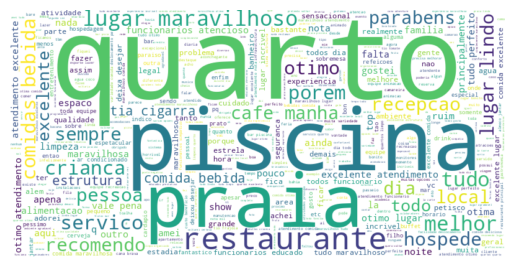
\includegraphics[width=1\textwidth]{figs/exploratoria/wordcloud_geral.png}
		\caption{Wordcloud sem stop words}
		\label{img:wordcloud_geral}
	\end{minipage}
\end{figure}

Já considerando a nuvem de palavras filtrando apenas por adjetivos teremos então na Figura \ref{img:wordcloud_adjetivos} que tem como alguns dos destaques palavras como sensacional, excelente, especial, local, top, ótimo, nota.

E por último observamos a nuvem de palavras levando em consideração apenas os substantivos na Figura \ref{img:wordcloud_substantivos}, que como destaque podemos citar funcionário, piscina, quarto, praia.

\begin{figure}
	\centering
	\begin{minipage}{0.45\textwidth}
		\centering
		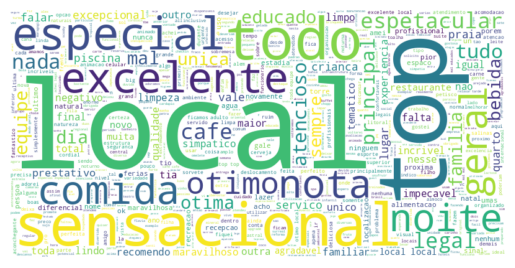
\includegraphics[width=1\textwidth]{figs/exploratoria/wordcloud_adjetivos.png}
		\caption{Wordcloud de Adjetivos}
		\label{img:wordcloud_adjetivos}
	\end{minipage}
	\begin{minipage}{0.45\textwidth}
		\centering
		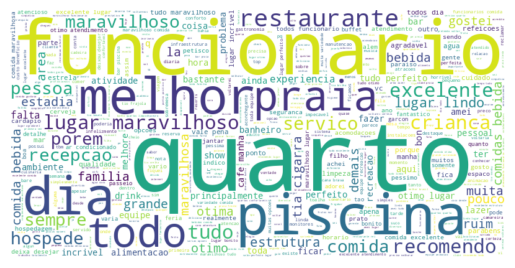
\includegraphics[width=1\textwidth]{figs/exploratoria/wordcloud_substantivos.png}
		\caption{Wordcloud de substantivos}
		\label{img:wordcloud_substantivos}
	\end{minipage}
\end{figure}

Outra forma de análise é o agrupamento de tokens em unigramas na Figura \ref{img:unigramas}, bigramas na Figura \ref{img:bigramas} e os trigramas na Figura \ref{img:trigramas} presentes em todas as avaliações. dessa forma temos exatamente a classificação de franquênia dos tokens no corpus de estudo.

Entre os unigramas \ref{img:unigramas} temos uma lista com alguns dos tokens mais frequentes, alguns chegando a passar a contagem de utilização de mais de 10.000 vezes, como é o caso de lugar, sendo seguindo ainda que próximo por comida, excelente e atendimento, este ultimo com uma frequência próximo de 8500 vezes. Ainda em relação aos unigramas também podemos levar em consideração a sua frequência com a evolução do tempo em \ref{img:rank_unigramas}, e algo com grande destaque é a palavra lugar que está entre o top 10 entre todo o período da análise, flutuando entre as cinco primeiras posições, tio é um unigrama que merece atenção, por não aparecer na nuvem de palavras de unigramas, porém se faz presente no ranking se observarmos individualmente os anos ele aparece em décimo lugar no ano de 2022, indícios de uma possível atração local bem conhecida, substituindo então o unigrama 'praia', que se fazia presente no ranking até 2021 na nona colocação.

\begin{figure}
	\centering
	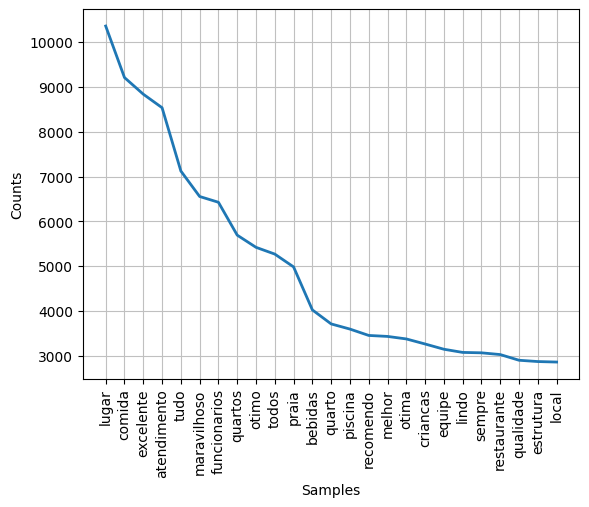
\includegraphics[width=.8\textwidth]{figs/exploratoria/unigramas.png}
	\caption{Unigramas}
	\label{img:unigramas}
\end{figure}

Considerando os bigramas \ref{img:bigramas} a frequência diminui consideravelmente, pois aqui temos que a ordem importa e dessa forma o mais frequente fica próximo de 1700 vezes, sendo composto pela dupla 'lugar' e 'maravilhoso', seguido pelo segundo colocado, bem próximo de 1400 vezes, sendo 'comida' e 'boa', onde podemos observar a grande frequência de palavras positivas, por conta dos adjetivos positivos.

\begin{figure}[!h]
	\centering
	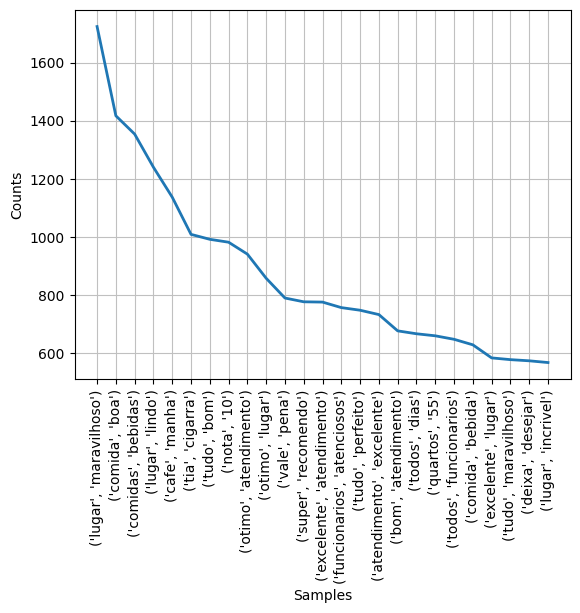
\includegraphics[width=.8\textwidth]{figs/exploratoria/bigramas.png}
	\caption{Bigramas}
	\label{img:bigramas}
\end{figure}

Para destaque entre os trigramas \ref{img:trigramas} a frequência diminui ainda mais e como destaque temos um que supera a contagem de 250 vezes, sendo 'facilidade', 'deslocamento' e 'pe', o que nos indica que existe pelo menos um hotel que possui uma boa localização para ser possível se deslocar até uma atração popular do local a pé, seguido de 'atendimento', 'nota' e '10' que indica que para as pessoas que avaliaram o atendimento da rede de hotéis ainda é algo importante e que deve ser levado em consideração caso a rede tenha interesse em ter ou manter um conceito positivo entre seus clientes.

\begin{figure}
	\centering
	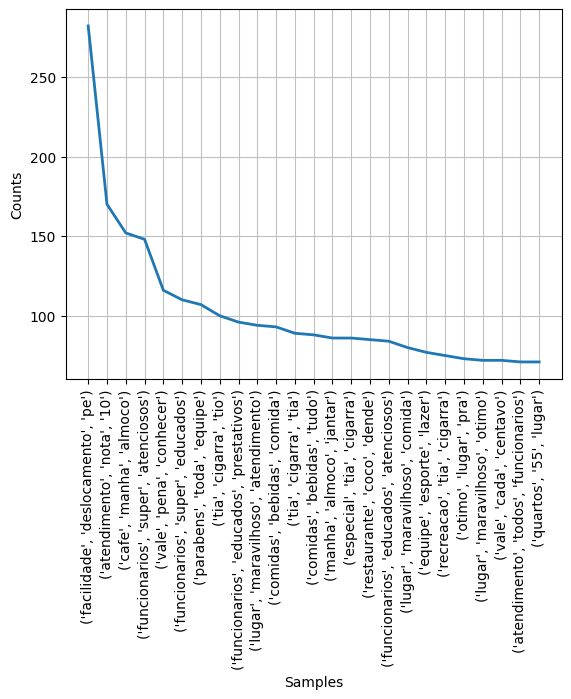
\includegraphics[width=.8\textwidth]{figs/exploratoria/trigramas.png}
	\caption{Trigramas}
	\label{img:trigramas}
\end{figure}

\begin{figure}
	\centering
	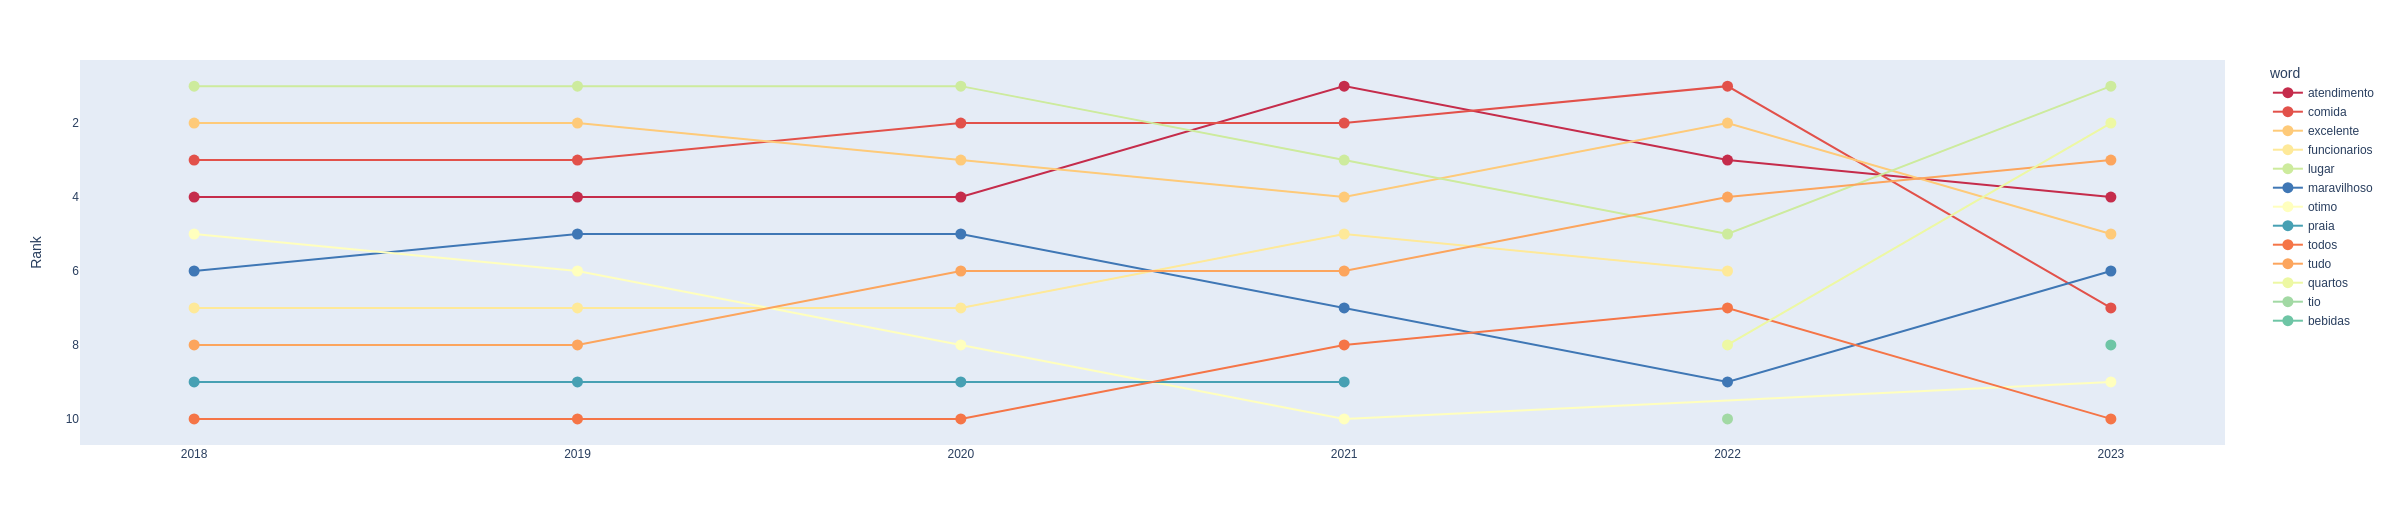
\includegraphics[width=1\textwidth]{figs/exploratoria/ranking_unigramas_por_ano.png}
	\caption{Ranking de unigramas por ano}
	\label{img:rank_unigramas}
\end{figure}

\section{Análise de Sentimentos Temporal}
\label{cap:resultados:sec:analise_sentimento}

\subsection[BERT]{BERT}
\label{sec:resultados:subsec:bert}

O tempo de execução médio, após 5 execuções cada, para que a análise de todo o corpus fosse realizada, foi o seguinte:

\begin{itemize}
	\item philschmid/distilbert-base-multilingual-cased-sentiment: 3min e 37s
	\item lxyuan/distilbert-base-multilingual-cased-sentiments-student: 3min e 36s
	\item citizenlab/twitter-xlm-roberta-base-sentiment-finetunned: 6min e 54s
	\item cardiffnlp/twitter-xlm-roberta-base-sentiment: 6min e 44s
	\item ramonmedeiro1/bertimbau-products-reviews-pt-br: 6min e 59s
\end{itemize}

Considerando apenas os \textit{BERTs} notamos um desempenho com relação à velocidade de execução bem interessante, levando em consideração que estamos utilizando um ambiente de execução para realizar os testes que possui um poder computacional razoável para os tempos modernos.

Após realizar o tratamento e levar em consideração o \textit{score} mais alto, temos quase 86\% das avaliações identificadas com o sentimento Positivo, em números absolutos 42078 avaliações, pouco mais de 6\% contendo sentimento Neutro e pouco mais de 8\% com sentimento negativo, como podemos observar na Figura~\ref{img:sentimento_bert}.

\begin{figure}
	\centering
	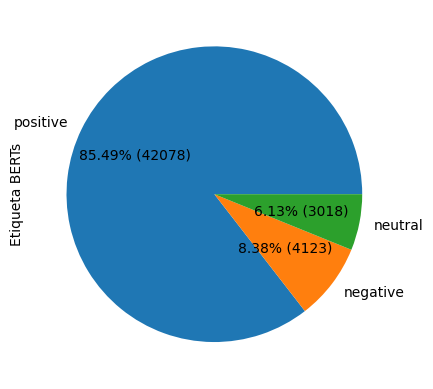
\includegraphics{figs/bert/distribuicao_pizza.png}
	\caption{BERTs - Distribuição do sentimento das avaliações}
	\label{img:sentimento_bert}
\end{figure}

Como já era esperado, a grande maioria das avaliações foram classificadas como sendo avaliações com sentimento positivo, em todos os anos, como é possível ser observado na Figura~\ref{img:sentimento_timechart_bert}.

Também conseguimos notar que quanto maior a nota maior a quantidade de avaliações com sentimento positivo, sendo que as avaliações com notas 4 e 5 contém uma discrepância grande com relação à quantidade de avaliações com sentimento positivo contra a quantidade de avaliações com sentimento neutro ou negativo, já as avaliações com nota 3 possuem uma distribuição mais equivalente e as avaliações com notas 1 e 2 com o sentimento negativo tendo grande destaque em relação às avaliações etiquetadas como neutro ou positivo, como é possível ser observado na Figura~\ref{img:sentimento_nota_bert}, que indica que os usuários tendem a dar uma nota mais elevada quando escrevem uma avaliação com um sentimento mais positivo.

\begin{figure}
	\centering
	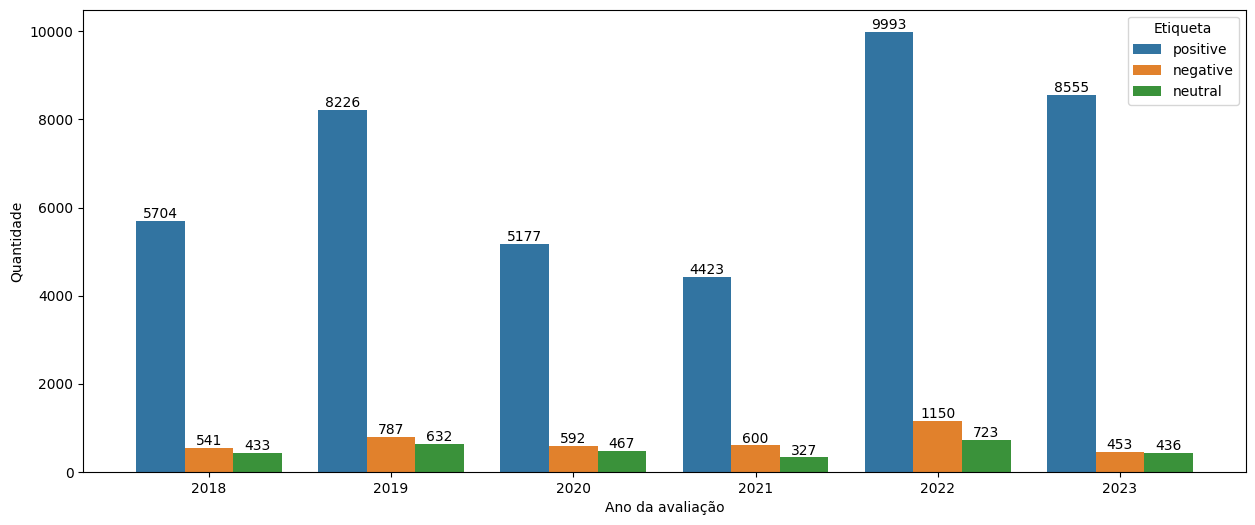
\includegraphics[width=1\textwidth]{figs/bert/sentimento_ano.png}
	\caption{BERTs - Sentimento das avaliações por ano}
	\label{img:sentimento_timechart_bert}
\end{figure}

\begin{figure}
	\centering
	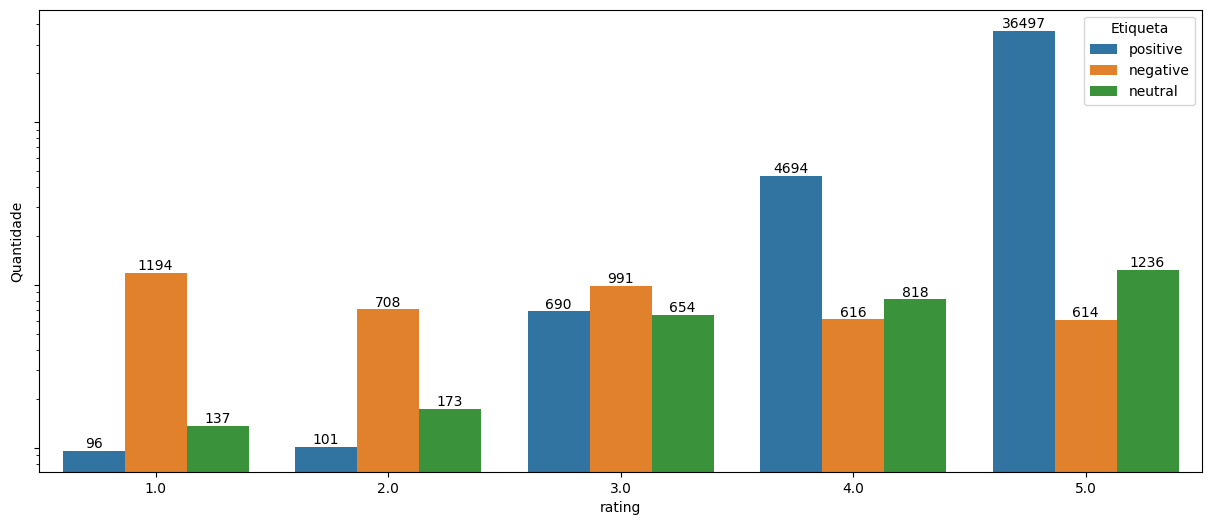
\includegraphics[width=1\textwidth]{figs/bert/sentimento_nota.png}
	\caption{BERTs - Sentimento das avaliações por nota}
	\label{img:sentimento_nota_bert}
\end{figure}

Porém, avaliando de forma individual cada um dos modelos, podemos notar uma grande discrepância entre eles, com a afinação mais eficiente para esse corpus sendo o do \textit{citizenlab}, considerando que eficiência aqui representa a maior número de avaliações classificadas com \textit{score} superior aos outros, como notamos na Figura \ref{img:rinha_de_berts}, modelo esse que levou menos de 7 minutos para executar e classificar todo o corpus, seguido pelo \textit{philschmid} que levou cerca de 3 minutos e meio na média.

\begin{figure}
	\centering
	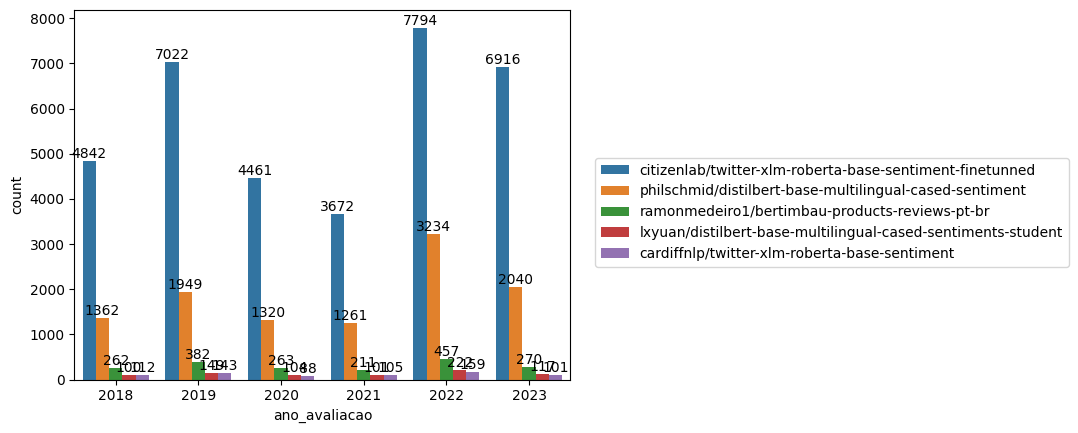
\includegraphics[width=1\textwidth]{figs/bert/desempenho_berts.png}
	\caption{BERTs - Quantidade de avaliações com maior \textit{score} por ano}
	\label{img:rinha_de_berts}
\end{figure}

Nas Figuras~\ref{img:sentimento_phil} e~\ref{img:sentimento_citizenlab} conseguimos visualizar a classificação atribuída de forma individual por ambos os modelos, a versão de \textit{philschmid} e \textit{citizenlab} respectivamente, com o \textit{citizenlab} classificando um número maior de sentimentos positivos, porém com um número de sentimentos neutros e negativos similar, o mesmo não acontece com \textit{philschmid} que tem um número maior de sentimentos neutros em comparação direta, porém da mesma forma um número de sentimento positivo maior e desigual.

\begin{figure}
	\centering
	\centering
	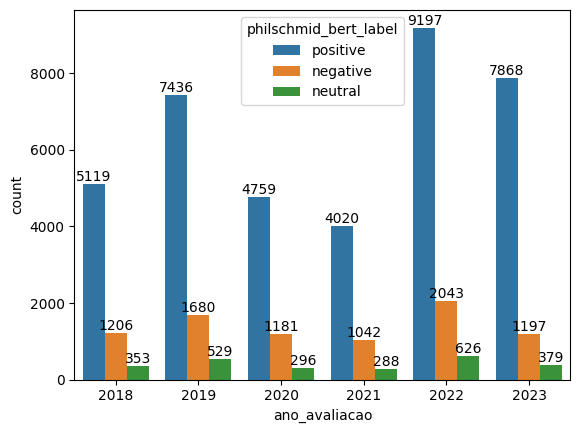
\includegraphics[width=1\textwidth]{figs/bert/classificacao_phil.png}
	\caption{BERT philschmid - Sentimento das avaliações por ano}
	\label{img:sentimento_phil}
\end{figure}

\begin{figure}
	\centering
	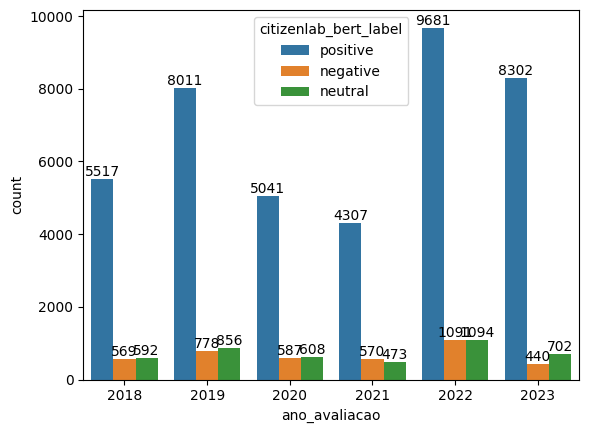
\includegraphics[width=1\textwidth]{figs/bert/classificacao_citizenlab.png}
	\caption{BERT citizenlab - Sentimento das avaliações por ano}
	\label{img:sentimento_citizenlab}
\end{figure}


Todos os modelos \textit{BERTs} etiquetam as avaliações de forma aparentemente consistente, como era esperado, temos uma quantidade muito grande de avaliações com nota máxima, 5, e por esse motivo é esperado que o sentimento geral das avaliações de nota 4 ou 5 seja positivo, avaliações com nota 3 distribuição de sentimento mais uniforme e as notas 1 e 2 contendo uma quantidade maior de sentimento negativo.

Os resultados indicam que os modelos \textit{BERTs} concordam com o modelo \textit{GPT} em quase 89\% das avaliações, conforme Figura \ref{img:bert_vs_gpt}, mostrando uma alta taxa de concordância geral entre os modelos na identificação de sentimentos. Essa elevada consistência sugere que ambos os modelos são eficazes na tarefa, especialmente em relação às avaliações positivas.

\begin{figure}
	\centering
	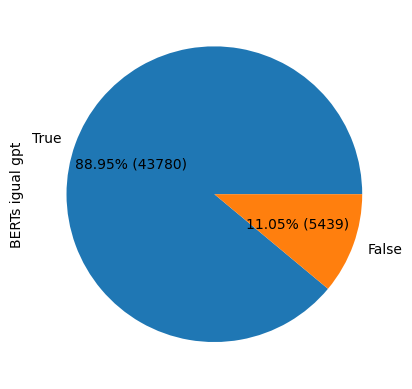
\includegraphics{figs/bert/vs_gpt.png}
	\caption{BERT com sentimento igual ao GPT}
	\label{img:bert_vs_gpt}
\end{figure}

No entanto, a Figura \ref{img:heat_bert_vs_gpt} revela áreas de discordância, principalmente nas avaliações negativas e neutras. Embora ambos os modelos concordem fortemente nas classificações positivas, com 40.224 avaliações coincidentes, há uma divergência considerável nas categorias negativas e neutras. Isso sugere que os modelos podem ter abordagens diferentes para sentimentos mais ambíguos ou menos claros, importante levar em consideração que o \textit{GPT} não conseguiu classificar todas as avaliações, falaremos mais sobre isso na seção do \textit{GPT}, em \ref{sec:resultados:subsec:gpt}.

\begin{figure}
	\centering
	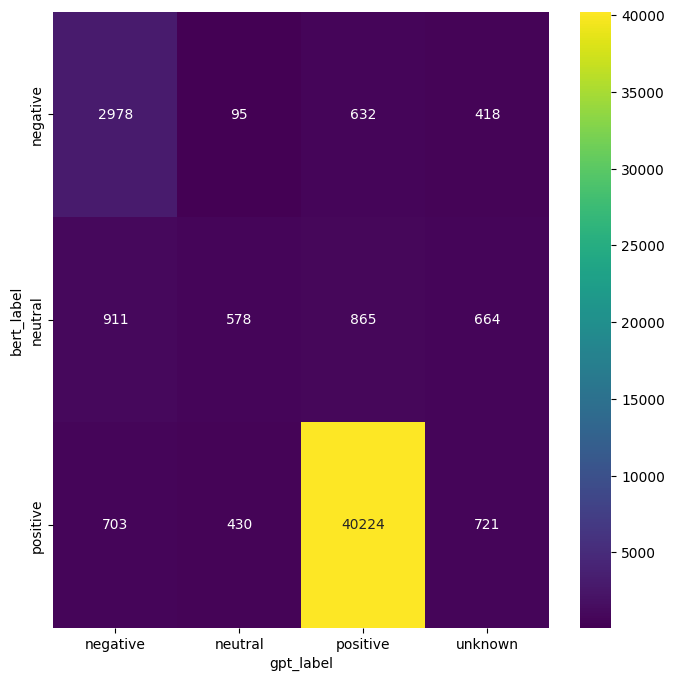
\includegraphics[width=.8\textwidth]{figs/bert/heat_vs_gpt.png}
	\caption{Distribuição de sentimento BERTs comparado com GPT}
	\label{img:heat_bert_vs_gpt}
\end{figure}


\subsection{Vicuna}
\label{sec:resultados:subsec:vicuna}


O modelo \textit{Vicuna} demorou pouco mais do que 6 horas para realizar a tarefa de atribuição de etiqueta para cada uma das avaliações, o que é pode ser um ponto negativo dependendo do projeto que se está executando, ele demorou um tempo consideravelmente maior se comparado com os modelos \textit{BERTs} e para a tarefa proposta no trabalho ambos realizaram uma simular em termos de volume de etiquetas atribuídas para as avaliações, ambos reconheceram como sendo positivas a grande parte, mais de 86\% das avaliações, e o segundo maior grupo como sendo as avaliações negativas, como observado na Figura \ref{img:vicuna_pizza_distribuicao}.

\begin{figure}
	\centering
	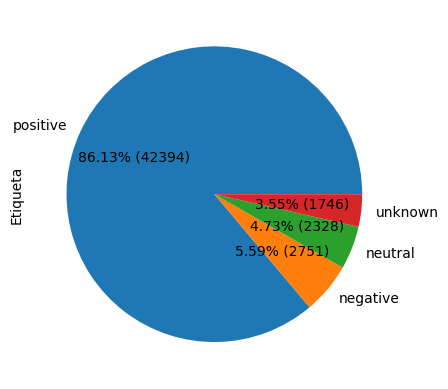
\includegraphics{figs/vicuna/distribuicao_pizza.png}
	\caption{Vicuna - Distribuição do sentimento das avaliações}
	\label{img:vicuna_pizza_distribuicao}
\end{figure}

Continuamos aqui com o mesmo comportamento de quantidade de avaliações com sentimento positivo brutalmente maior se comparado com os outros sentimentos, porém também temos agora o cenário onde o modelo não conseguir realizar a tarefa com sucesso e atribuir uma etiqueta apropriada a avaliação, dessa forma elas foram etiquetadas com o valor \textit{UNKNOWN}, temos 1746(3.55\%) avaliações nesse estado, cenário que não temos com os modelos \textit{BERT}, que considerando a quantidade total de avaliações pode ser considerado um número baixo, porém se avaliarmos ano a ano, a quantidade de avaliações com esse valor de etiqueta acaba se tornando relevante, até mesmo em quantidade superiores aos outros sentimentos (neutro e negativo), como observado na Figura \ref{img:vicuna_sentimento_ano}, mas mesmo assim o \textit{Vicuna} atribuiu algum sentimento para a maioria das avaliações, sendo o grupo de avaliações com problema na classificação o grupo com menor quantidade de avaliações.

\begin{figure}
	\centering
	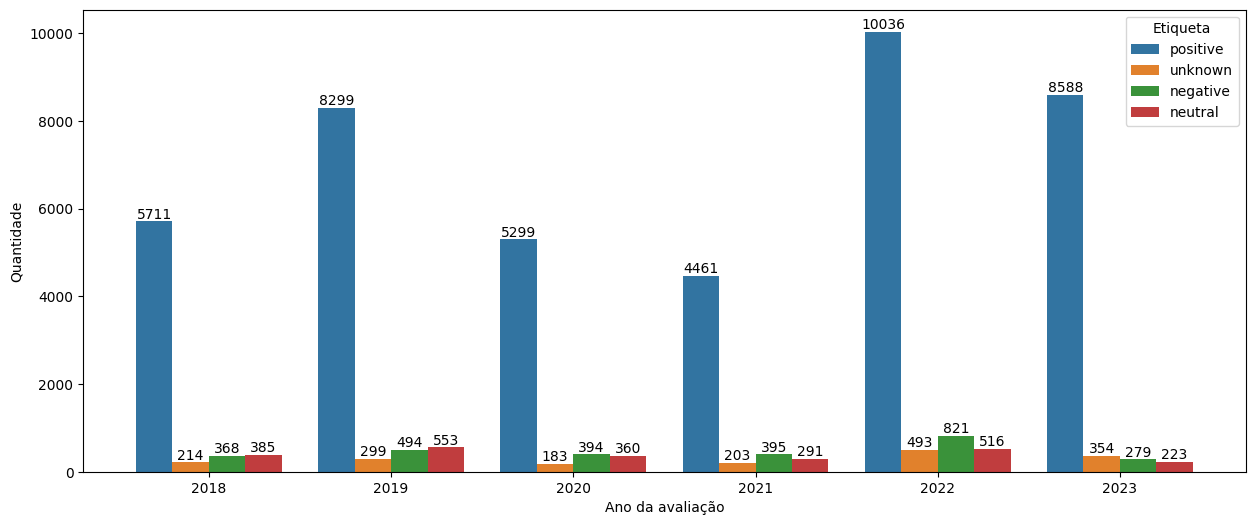
\includegraphics[width=1\textwidth]{figs/vicuna/sentimento_ano.png}
	\caption{Vicuna - Sentimento das avaliações por ano}
	\label{img:vicuna_sentimento_ano}
\end{figure}

Olhando especificamente para a distribuição por nota atribuída temos um comportamento ainda mais curioso ao observar a nota 3, onde todas as etiquetas possuem uma quantidade equivalente e bem próxima, o comportamento de notas 1 e 2, de possuir uma quantidade de avaliações com sentimento negativo superior as outras etiquetas juntas, e temos o mesmo comportamento para as notas 4 e 5, porém o sentimento que supera é o positivo, como observado pela Figura \ref{img:vicuna_sentimento_nota}.

\begin{figure}
	\centering
	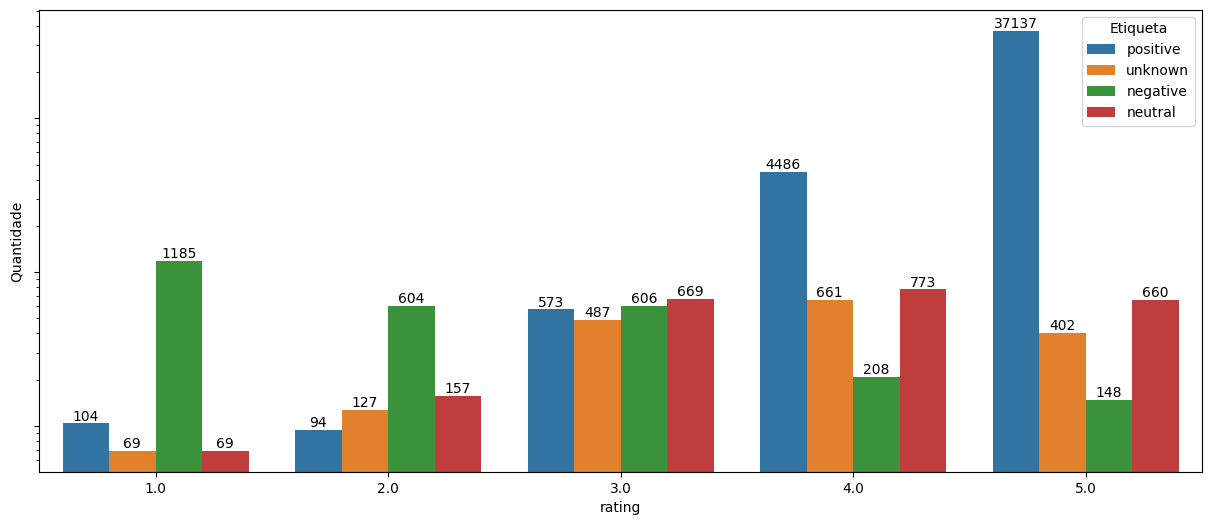
\includegraphics[width=1\textwidth]{figs/vicuna/sentimento_nota.png}
	\caption{Vicuna - Sentimento das avaliações por nota}
	\label{img:vicuna_sentimento_nota}
\end{figure}

Os resultados indicam que o \textit{Vicuna} concordam com o modelo \textit{GPT} em quase 89\% das avaliações, conforme Figura \ref{img:vicuna_vs_gpt}, mostrando uma alta taxa de concordância geral entre os modelos na identificação de sentimentos. Essa elevada consistência sugere que ambos os modelos são eficazes na tarefa, especialmente em relação às avaliações positivas.

\begin{figure}
	\centering
	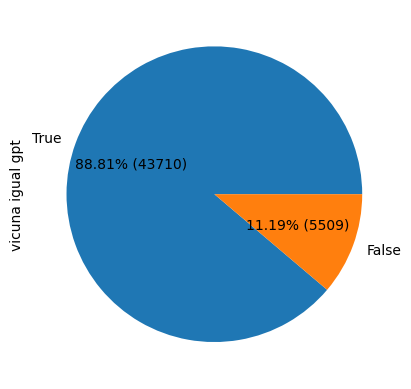
\includegraphics{figs/vicuna/vs_gpt.png}
	\caption{Vicuna com sentimento igual ao GPT}
	\label{img:vicuna_vs_gpt}
\end{figure}

No entanto, a Figura \ref{img:heat_vicuna_vs_gpt} revela áreas de discordância, principalmente nas avaliações negativas, neutras e as que ambos não conseguiram classificar. Embora ambos os modelos concordem fortemente nas classificações positivas, com 40.425 avaliações coincidentes, há uma divergência considerável nas outras categorias, com destaque para as avaliações onde o \textit{Vicuna} classificou como neutro e o \textit{GPT} classificou como negativo. Isso sugere que os modelos podem ter abordagens diferentes para sentimentos mais ambíguos ou menos claros.

\begin{figure}
	\centering
	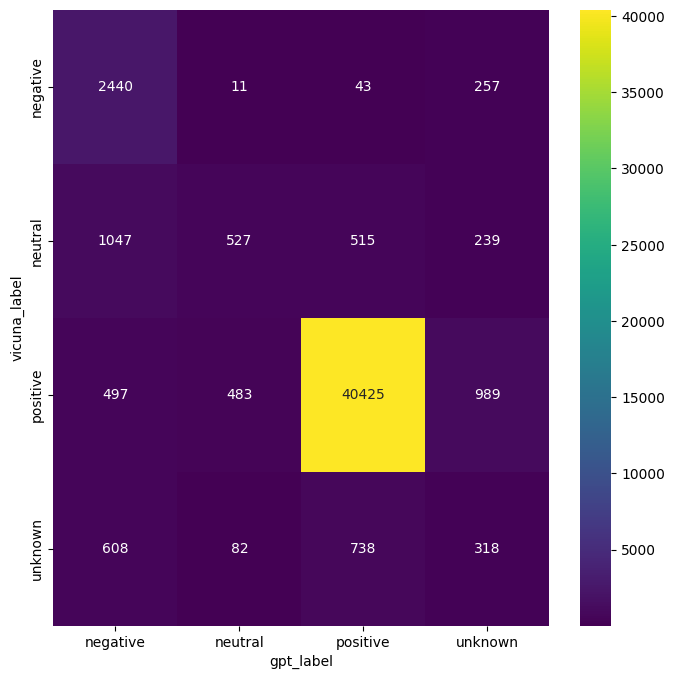
\includegraphics[width=.8\textwidth]{figs/vicuna/heat_vs_gpt.png}
	\caption{Distribuição de sentimento Vicuna comparado com GPT}
	\label{img:heat_vicuna_vs_gpt}
\end{figure}


\subsection{GPT 3.5}
\label{sec:resultados:subsec:gpt}

%TODO revisar imagens

O modelo \textit{GPT} 3.5 demorou pouco mais do que 4 horas e teve custo de pouco menos de 11 dólares para realizar a tarefa de atribuição de etiqueta para cada uma das avaliações, além de ser um modelo pago e privado, o que é pode ser um ponto negativo dependendo do projeto que se está executando, ele demorou um tempo consideravelmente maior se comparado com os modelos \textit{BERTs} e para a tarefa proposta no trabalho ambos realizaram uma simular em termos de volume de etiquetas atribuídas para as avaliações, ambos reconheceram como sendo positivas a grande parte, mais de 84\% das avaliações, e o segundo maior grupo como sendo as avaliações negativas.

Outra grande desvantagem do \textit{GPT} é que se faz necessário uso de rede de internet nesse caso, por conta do modelo ser executado na nuvem da OpenAI, que acaba por gerar exposição desnecessária dos dados se comparado com modelos abertos que podem ser executados sem a necessidade de utilização da internet.

Utilizando o modelo GPT 3.5 para realizar a tarefa de análise de sentimentos do conteúdo textual das avaliações obtemos a distribuição conforme Figura \ref{img:gpt_pizza_distribuicao}, onde 84.77\% das avaliações, ou seja, 41721 avaliações foram classificadas como tendo um sentimento positivo, isso representa um número próximo das avaliações que receberam como nota 4 ou 5, 6128 e 38347 avaliações respectivamente, porém fica fácil notar na Figura \ref{img:gpt_sentimento_nota} que mesmo a grande maioria das avaliações com essa nota atribuída ainda existem avaliações com sentimentos diferentes e até mesmo avaliações em quais a etiqueta atribuída não foi identificável, sendo assim marcadas como com a etiqueta \textit{UNKNOWN}, que foram classificadas dessa forma por conta do modelo não conseguir realizar a tarefa que lhe foi atribuída e produzir resposta maior ou mais detalhada sobre a etiqueta, e como o interesse é em classificações simples e diretas a etiqueta atribuída não foi identificável, mas diferente do que aconteceu com o \textit{Vicuna}, o \textit{GPT} teve mais dificuldade e não foi possível identificar o sentimento atribuído para mais avaliações do que o seu concorrente(1803 vs 1746), sendo o grupo de avaliações com problema na classificação um grupo com maior quantidade de avaliações, 1803(3.66\%) se comparado com o grupo de sentimento neutro, 1103(2.24\%).

\begin{figure}
	\centering
	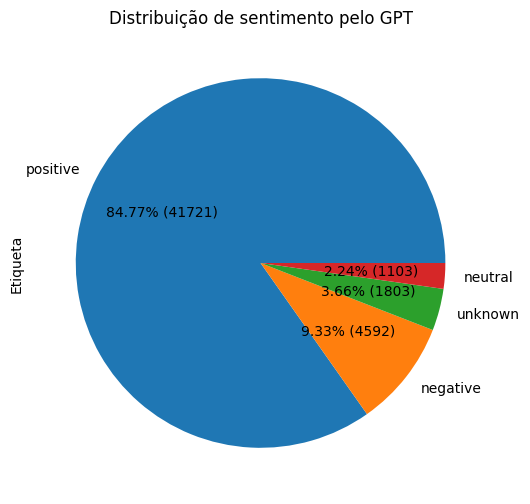
\includegraphics{figs/gpt/distribuicao_pizza.png}
	\caption{GPT - Distribuição do sentimento das avaliações}
	\label{img:gpt_pizza_distribuicao}
\end{figure}
\begin{figure}
	\centering
	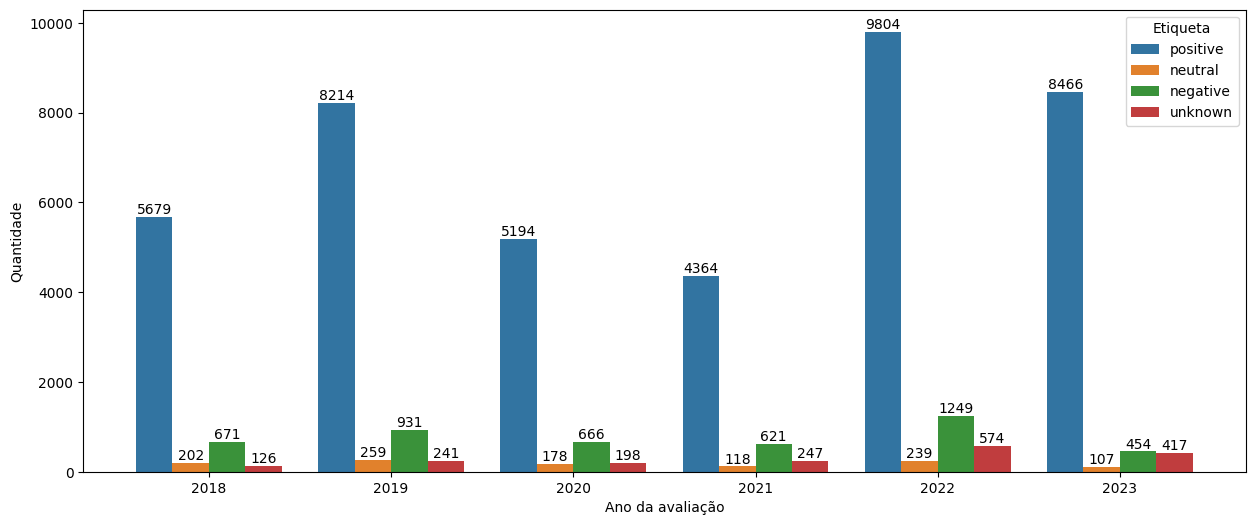
\includegraphics[width=1\textwidth]{figs/gpt/sentimento_ano.png}
	\caption{GPT - Sentimento das avaliações por ano}
	\label{img:gpt_sentimento_ano}
\end{figure}
\begin{figure}
	\centering
	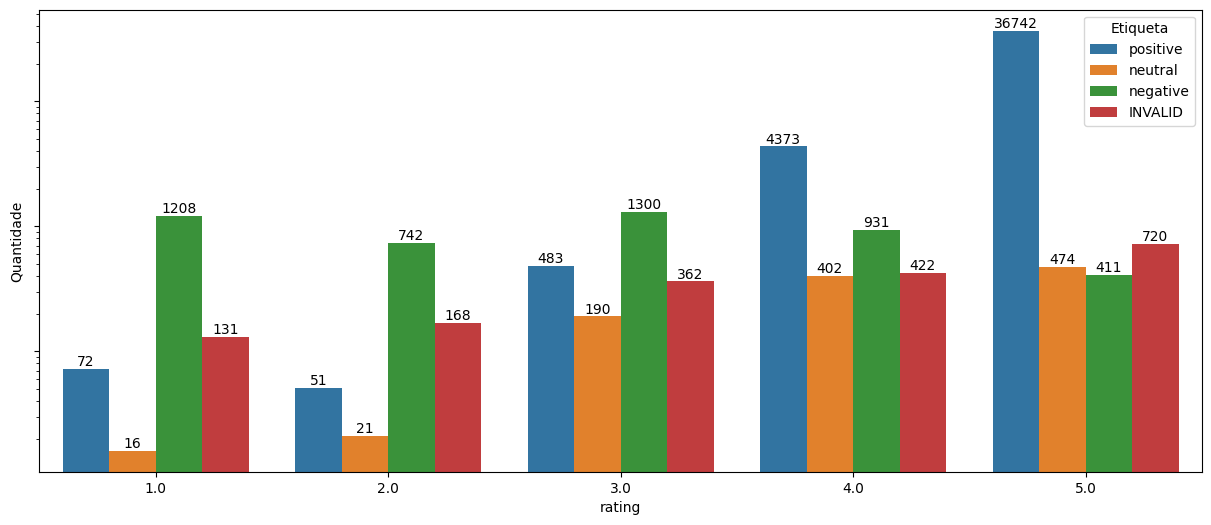
\includegraphics[width=1\textwidth]{figs/gpt/sentimento_nota.png}
	\caption{GPT - Sentimento das avaliações por nota}
	\label{img:gpt_sentimento_nota}
\end{figure}


\subsection{OpenChat}
\label{sec:resultados:subsec:openchat}

%TODO revisar imagens

O modelo OpenChat demorou aproximadamente 9 horas para realizar a tarefa de atribuição de etiqueta para cada uma das avaliações, por ser um modelo menor é esperado que seu desempenho seja inferior se comparado com os anteriores, seu tamanho menor pode ser também um ponto positivo por conta de serem necessários uma menor quantidade de memória de vídeo para carregar o modelo e conseguir realizar a execução do mesmo, ele demorou um tempo consideravelmente maior se comparado com todas as outras abordagens do projeto e para a tarefa proposta no trabalho a atribuição ainda foi simular, reconheceu como sendo positivas a grande parte, aproximadamente 83\% das avaliações, porém o grande destaque está no segundo maior grupo, que é o das avaliações que não foram possíveis classificar, com pouco mais de 11\%.

É perceptível que o modelo do OpenChat não conseguir executar um bom trabalho com o texto que inicia a tarefa se comparado com os outros LLMs, porém ele matem o comportamento esperado de ter um número de avaliações com sentimento positivo bastante destoante dos outros grupos.

Analisando algumas das classificações que o OpenChat realizou, especificamente contendo o texto \textit{Sem palavras}, temos o total de 7 avaliações com o mesmo texto, todas com uma nota de 5 estrelas atribuída pelo usuário, que não foi levada em consideração no momento de análise, o que é interessante notar é que o GPT classifica todas como sendo de sentimento neutro, já o \textit{Vicuna} classifica como sendo sentimento positivo, porém o OpenChat classifica 5 como tendo o sentimento positivo e as outras duas como sendo de sentimento neutro, o que pode indicar que o ambiente de testes não estava devidamente configurado para que a reprodutividade com esse modelo fosse algo consistente ou que o modelo tem certa inconsistência.

\begin{figure}
	\centering
	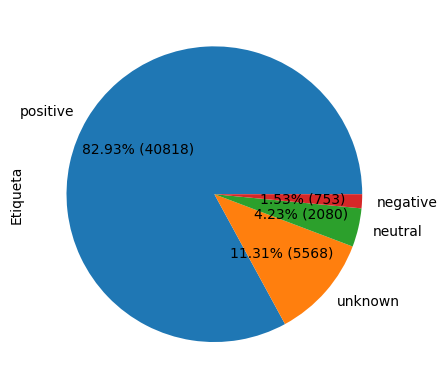
\includegraphics{figs/openchat/distribuicao_pizza.png}
	\caption{OpenChat - Distribuição do sentimento das avaliações}
	\label{img:openchat_pizza_distribuicao}
\end{figure}

\begin{figure}
	\centering
	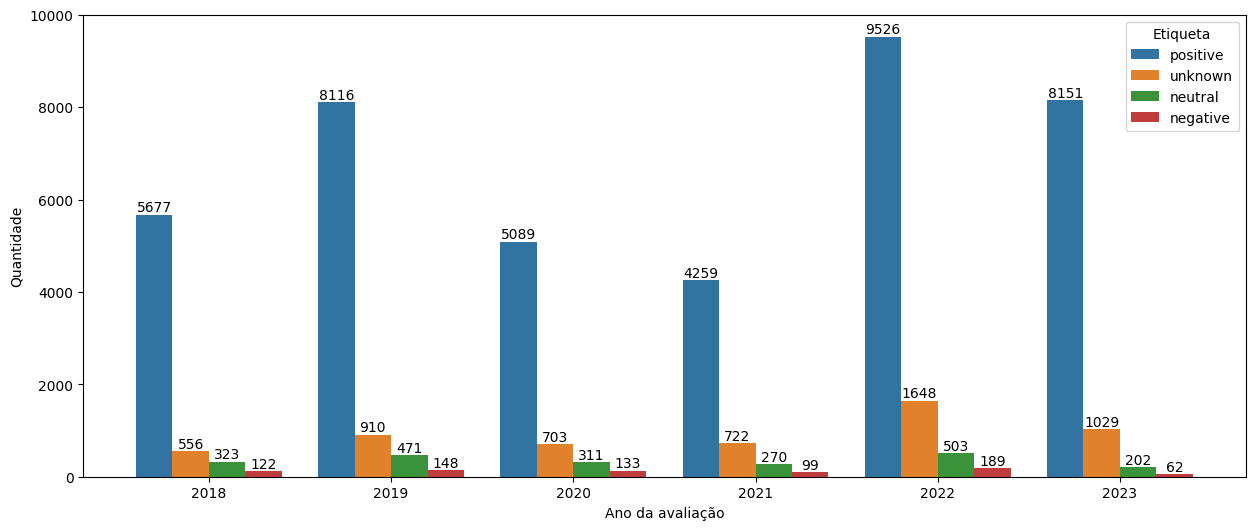
\includegraphics[width=1\textwidth]{figs/openchat/sentimento_ano.png}
	\caption{OpenChat - Sentimento das avaliações por ano}
	\label{img:openchat_sentimento_ano}
\end{figure}

\begin{figure}
	\centering
	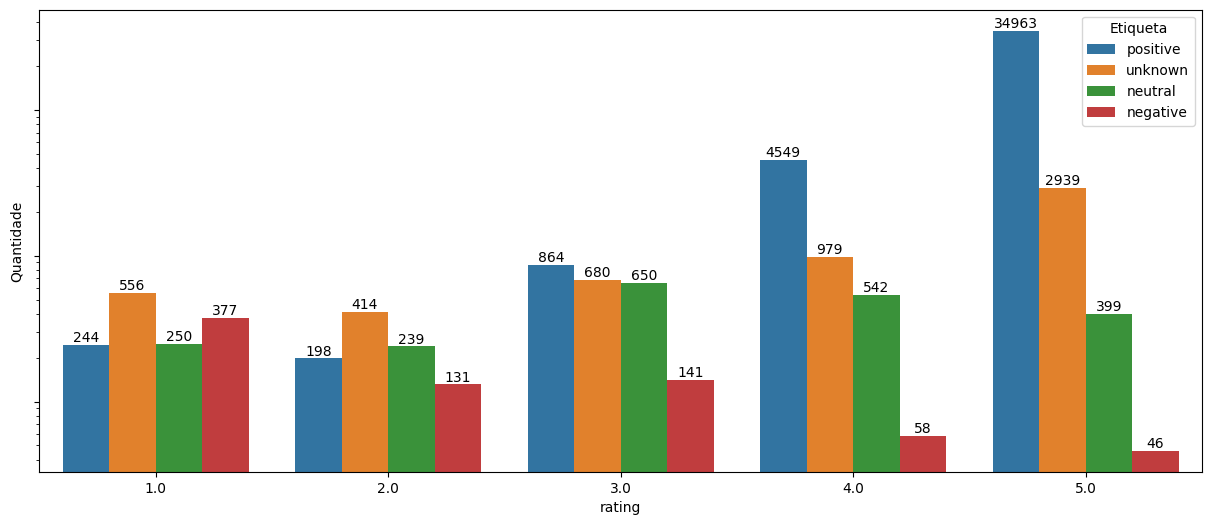
\includegraphics[width=1\textwidth]{figs/openchat/sentimento_nota.png}
	\caption{OpenChat - Sentimento das avaliações por nota}
	\label{img:openchat_sentimento_nota}
\end{figure}

HEAT MAPS.

\begin{figure}
	\centering
	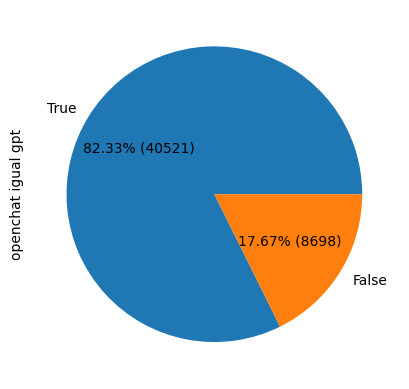
\includegraphics{figs/openchat/vs_gpt.png}
	\caption{OpenChat com sentimento igual ao GPT}
	\label{img:openchat_vs_gpt}
\end{figure}

\begin{figure}
	\centering
	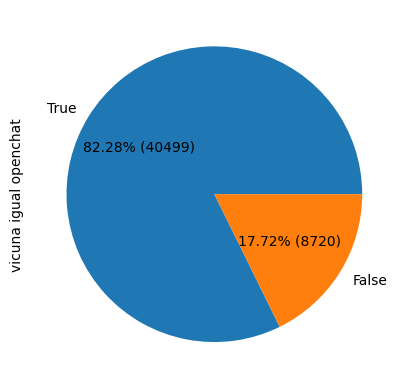
\includegraphics{figs/openchat/vs_vicuna.png}
	\caption{OpenChat com sentimento igual ao Vicuna}
	\label{img:openchat_vs_vicuna}
\end{figure}

\begin{figure}
	\centering
	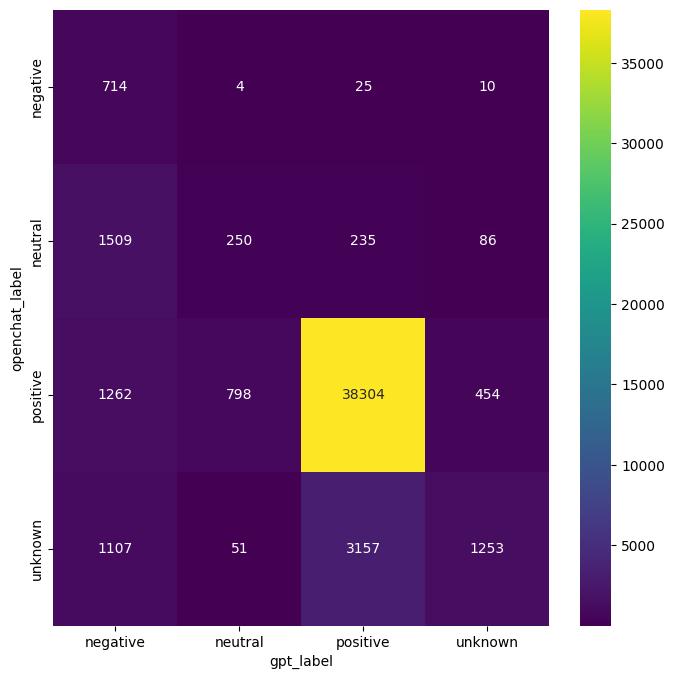
\includegraphics[width=.8\textwidth]{figs/openchat/heat_vs_gpt.png}
	\caption{Distribuição de sentimento OpenChat comparado com GPT}
	\label{img:heat_openchat_vs_gpt}
\end{figure}

\begin{figure}
	\centering
	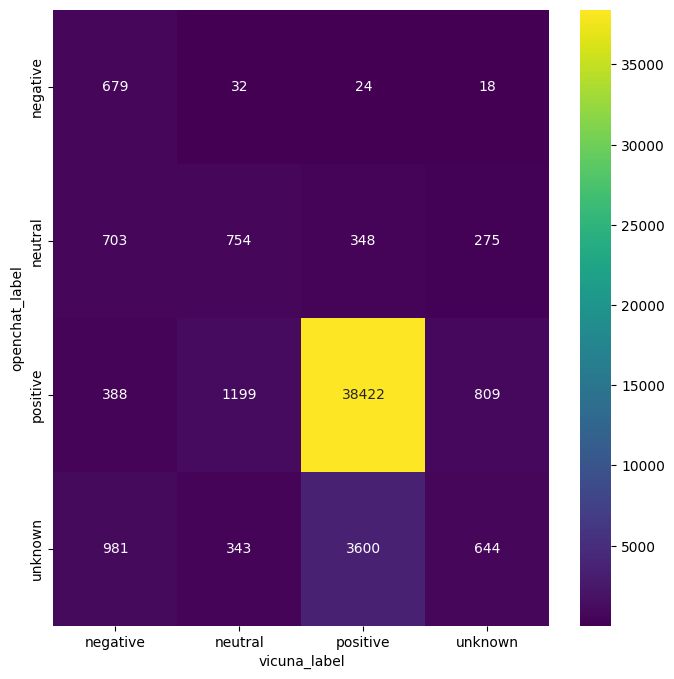
\includegraphics[width=.8\textwidth]{figs/openchat/heat_vs_vicuna.png}
	\caption{Distribuição de sentimento OpenChat comparado com Vicuna}
	\label{img:heat_openchat_vs_vicuna}
\end{figure}

\begin{figure}
	\centering
	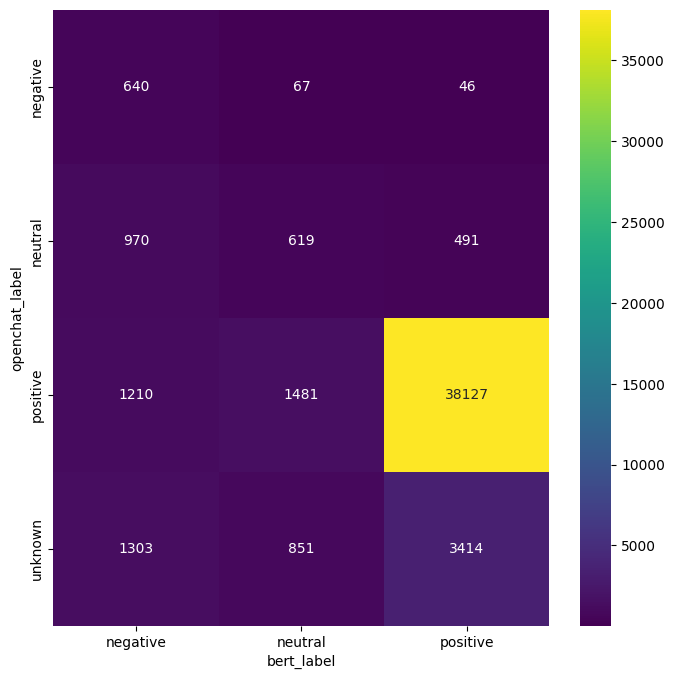
\includegraphics[width=.8\textwidth]{figs/openchat/heat_vs_bert.png}
	\caption{Distribuição de sentimento OpenChat comparado com BERTs}
	\label{img:heat_openchat_vs_bert}
\end{figure}



% bert vs GPT
